Обозначим оптимальное значение, как
\begin{equation}
	OPT = \min_{\pi \in S_n} cost(\pi)
\end{equation}

\subsection{Минимальное остовное дерево}

Остов (остовное дерево) --- это подграф $ T = (V, E_T) $ , где:
\begin{itemize}
	\item $ |E_T| = n - 1 $ ;
	\item граф $T$ связен
\end{itemize}

Вес остовного дерева определяется через функцию весов исходного графа $ G $:
\begin{equation}
	w(T) = \sum_{e \in E_T} d(e)
\end{equation}

Минимальное остовное дерево --- остов графа, имеющий минимальный возможный вес.

\begin{equation}
	T^{*} = \arg \min_T w(T)
\end{equation}

Построив минимальное остовное дерево (MST), совершим обход в глубину по этому дереву, записывая вершины в порядке посещения. Удалив из этого обхода возвращения в уже посещенные вершины, получим перестановку $\pi$ --- гамильтонов путь, являющийся 2-аппроксимацией решения TSP на изначальном графе.

\section{Доказательство минимальной точности аппроксимации, достигаемой при применении минимального остовного дерева для решения TSP}

\begin{lemma}
	$$
		w(T^{*}) \leq OPT
	$$
\end{lemma}
\begin{proof}
	Пусть $ C^{*} $ --- оптимальный цикл (то есть --- решение TSP для данного графа $ G = (V, E) $ ). Тогда:
	$$
		C^{*} \subseteq E
	$$
	Удалим одно ребро $e$ из $ C^{*} $. Получим связный граф с $n-1$ ребрами --- то есть остов $T$.
	$$
		w(T) = OPT - d(e) \leq OPT
	$$
	Так как $ w(T^{*}) $ минимален:
	$$
		w(T^{*}) \leq w(T) \leq OPT
	$$
\end{proof}

\subsection{Конструкция 2-аппроксимации}

Построим $ T^{*} $.

Определим мультимножество ребер:

$$
	E' = E_{T^{*}} \cup E_{T^{*}}
$$

Получим мультиграф:

$$
	G' = (V, E')
$$

Тогда

$$
	\forall v \in V \quad \deg_{G'}(v) = 2 \deg_{T^{*}} (v)
$$

Следовательно, $ \forall v \in V \quad \deg_{G'}(v) $ четна.

Так как граф $G$ связен, то связен и мультиграф $G'$, следовательно для него существует эйлеров цикл. Обозначим его как

$$
	W = (v_1, \dots, v_{2n-1}, v_1)
$$

Эйлеров обход $W$ дважды использует каждое ребро, поэтому:
$$
	w(W) = 2w(T^{*})
$$

Определим отображение

$$
	\phi : \{1, \dots, k\} \to V
$$

где $ \phi (i) $ --- $  i  $-я вершина эйлерова обхода.

Построим последовательноесть без повторов:
$$
	\sigma = (\sigma_1, \dots, \sigma_n)
$$

по следующему принципу:
\begin{itemize}
	\item $\sigma_1 = \phi(1)$;
	\item далее, будем включать вершины только при первом их появлении.
\end{itemize}

В результате получим биекцию:
\[
	\sigma: \{ 1, \dots, n \} \to V
\]

\begin{lemma}
	\[
		cost(\sigma) \leq w(W)
	\]
\end{lemma}
\begin{proof}
	Пусть в обходе встречается фрагмент:
	\[
		u \to v \to w
	\]
	Если вершина $v$ уже посещена, заменяем его на:
	\[
		u \to w
	\]
	По неравенству треугольника:
	\[
		d(u, w) \leq d(u, v) + d(v, w)
	\]
	Следовательно:
	\[
		cost(\sigma) \leq w(W)
	\]
\end{proof}

\begin{figure}[h]
	\centering
	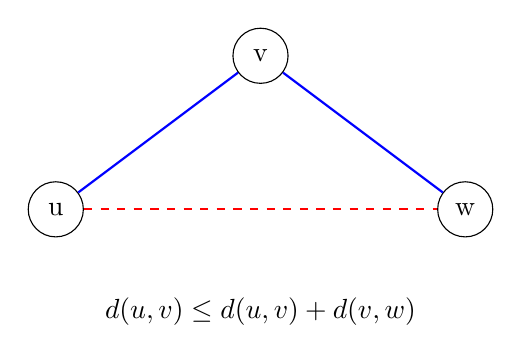
\begin{tikzpicture}[scale=1.3]
		\tikzstyle{vertex}=[circle,draw,minimum size=7mm]

		\node[vertex] (A) at (0,0) {u};
		\node[vertex] (B) at (2,1.5) {v};
		\node[vertex] (C) at (4,0) {w};

		\draw[thick, blue] (A) -- (B);
		\draw[thick, blue] (B) -- (C);

		\draw[thick, red, dashed] (A) -- (C);
		\node at (2, -1) {$d(u, v) \le d(u, v) + d(v, w)$};
	\end{tikzpicture}
	\caption{Использование неравенства треугольника при построении $\sigma$}
\end{figure}

В итоге получаем цепочку:
\[
	cost(\sigma) \leq w(W) = 2w(T^{*}) \leq 2 OPT
\]

Значит такой алгоритм является 2-аппроксимацией.
